\documentclass[acmsmall,nonacm,screen]{acmart}
\citestyle{acmauthoryear}

\usepackage{booktabs}
\usepackage{multirow}
\usepackage{seqsplit}
\usepackage{tikz}
\usetikzlibrary{arrows.meta,positioning,fit,decorations.pathreplacing,calc}
\usepackage{pgfplots}
\pgfplotsset{compat=1.18}
\usepgfplotslibrary{groupplots}
\usepackage[ruled,vlined,linesnumbered]{algorithm2e}

\AtEndPreamble{%
  \theoremstyle{acmdefinition}%
  \newtheorem{remark}[theorem]{Remark}}

\newcommand{\A}{\mathcal{A}}
\newcommand{\Lim}{\mathrm{Lim}}
\newcommand{\sigin}{\sigma^{\mathrm{in}}}
\newcommand{\upsin}{\upsilon^{\mathrm{in}}}
\newcommand{\act}{\mathrm{act}}
\newcommand{\Op}[1]{\textsc{#1}}
\makeatletter
\newcommand{\inputrows}[1]{\@@input #1 }
\makeatother

% Generated by scripts/summarize_fuzz.py; do not edit.
\newcommand{\FuzzTests}{13}
\newcommand{\FuzzRunsPerTest}{1{,}300}
\newcommand{\FuzzDepth}{256}
\newcommand{\FuzzCallsText}{4{,}326{,}400}
\newcommand{\FuzzLoans}{260{,}511}
\newcommand{\FuzzDefaults}{118{,}935}
\newcommand{\FuzzSlashing}{27{,}447}
\newcommand{\FuzzCharging}{16{,}793}
\newcommand{\FuzzResidual}{78{,}111}
\newcommand{\FuzzSybilLoans}{52{,}109}
\newcommand{\FuzzSybilDefaults}{25{,}874}
\newcommand{\FuzzSybilBacksOk}{1}
\newcommand{\FuzzSybilBacksRejected}{2{,}311{,}491}
\newcommand{\FuzzMaxQ}{100.00}
\newcommand{\FuzzMaxI}{99.98}

% Generated by scripts/mutation_summary.py; do not edit.
\newcommand{\MutationSummary}{Fuzzing detected eleven of the fourteen faults under every seed. The unit tests detected the remaining three.}


\begin{document}

\title{Conserved Credit: Sybil-Proof Loss Bounds for Uncollateralized Lending with Free Identities}
\subtitle{Working paper}

\author{Claude Code}
\affiliation{%
  \institution{Microcredit Protocol Project}
  \country{International}}
\authornote{Claude Code is an AI agent made by Anthropic. The research was directed by the project's human operator. See the disclosure at the end of the paper.}

\authorsaddresses{}

\begin{abstract}
The widely used lending protocols on public blockchains, Compound and Aave among them, require
collateral worth more than the loan, because accounts cost nothing to create and a protocol cannot
tell one person from many. We study a lending
pool that never infers creditworthiness from the structure of a trust graph. Every unit of
borrowing capacity is instead a liability of a named account: a line granted by an accountable
issuer, dues the account itself has paid into a first-loss reserve, or cash it has staked. An
account may back another by committing such credit, and a default charges the committed credit
before it reaches lenders. We prove that in every reachable state, lenders' realised loss plus their
loss on open loans is at most the issued lines plus the dues paid. Consequently, the loss a coalition
can cause is at most the credit issued inside it plus the unsecured backing that has ever been
committed to it from outside, whatever the number of accounts it controls. When lines change, the bound holds for each account's
highest line since the line was last unused, and not for current lines; this determines how an
issuer's budget must be charged. We also prove that any rule granting credit for repayment history
beyond the value that history irrevocably surrendered can be farmed for profit linear in the number
of accounts. This yields a trilemma between free identities, credit from history, and a bounded
loss. The protocol is implemented as a smart contract. Stateful fuzzing of the implementation
against an independent model, \FuzzCallsText{} calls in all, found no violation, and random
executions reached \FuzzMaxI\% of the loss bound.
\end{abstract}

\begin{CCSXML}
<ccs2012>
<concept><concept_id>10003752.10010070.10010099.10010101</concept_id>
<concept_desc>Theory of computation~Algorithmic mechanism design</concept_desc>
<concept_significance>500</concept_significance></concept>
<concept><concept_id>10002978.10003029.10003031</concept_id>
<concept_desc>Security and privacy~Economics of security and privacy</concept_desc>
<concept_significance>300</concept_significance></concept>
</ccs2012>
\end{CCSXML}
\ccsdesc[500]{Theory of computation~Algorithmic mechanism design}
\ccsdesc[300]{Security and privacy~Economics of security and privacy}

\keywords{Sybil attacks, sybilproof mechanisms, credit networks, uncollateralized lending, joint liability, decentralized finance}

\maketitle

% ---------------------------------------------------------------------------------------------
\section{Introduction}\label{sec:intro}

The widely used lending protocols on public blockchains, Compound and Aave among them, are
overcollateralised: a borrower locks assets worth more than the loan, and a smart contract sells
them if their value falls \citep{leshner2019compound,aave2020}. The requirement follows from the
setting. Accounts cost
nothing to create and carry no identity, so a protocol that extended unsecured credit to one account
would extend it to every account an attacker can create \citep{douceur2002sybil}. On-chain credit
is therefore available only to those who already hold assets. It is unavailable to borrowers
without collateral, without a credit history or without access to stable banking, who are the
borrowers that microcredit set out to serve.

Off-chain, unsecured credit to such borrowers often rests on a third party's word: a guarantor, a
group whose members are jointly liable, or a loan officer who knows the borrower
\citep{stiglitz1990peer,besley1995group,ghatak1999joint}. The obvious on-chain analogue is a trust
graph, in which accounts vouch for one another and creditworthiness is computed from the graph. That
analogue fails. No symmetric reputation function of a graph is sybilproof
\citep{cheng2005sybilproof}, and PageRank can be raised by a ring of fabricated accounts
\citep{cheng2006pagerank}. A predecessor of the protocol studied here computed credit with
personalised PageRank over attestations. Adversarial testing found rings of new accounts that
borrowed more than honest users (Section~\ref{sec:sim}).

This paper takes a different route. The protocol never infers creditworthiness from the shape of
the graph. Every unit of borrowing capacity is a liability of a named account, drawn from one of
three sources: a line granted by an issuer that answers for it, dues the account has itself paid
into a first-loss reserve, or cash the account has staked. Backing another account moves capacity
from the backer to the borrower and commits the backer's credit to the borrower's loans; it never
creates capacity. When a borrower defaults, the loss falls first on secured backing, whose stake is
slashed, then on unsecured backing, whose credit is burned, then on a reserve, and only then on
lenders. In the terms of \citet{litos2017trust}, trust is risk: an account can extend trust only up
to what it stands to lose.

That a trust graph becomes robust when its edges carry liability is an old idea. It underlies
TrustDavis \citep{defigueiredo2005trustdavis} and credit networks
\citep{ghosh2007trust,karlan2009trust,dandekar2011liquidity}. What this paper adds is a set of exact
loss bounds for a concrete protocol, with proofs that cover every reachable state of the
implemented state machine. The proofs cover partial repayment, several open loans per borrower,
defaults of backers, revocation of backing and changes to issued lines. The paper also proves an
impossibility result that fixes how much credit on-chain repayment history may earn.

\paragraph{Contributions.}
\begin{itemize}
\item A model of a lending pool with one-hop backing, coverage-discounted unsecured backing and a
  default waterfall (Section~\ref{sec:model}).
\item \emph{Conservation of capacity} (Theorem~\ref{thm:capacity}). Total borrowing capacity never
  exceeds granted credit plus committed stake, so the capacity of a coalition does not grow with
  the number of accounts in it (Corollary~\ref{cor:coalition-capacity}).
\item \emph{A loss bound over time} (Theorem~\ref{thm:loss}). In every reachable state, lenders'
  realised loss plus their potential loss on open loans is at most the issued lines plus the dues
  paid. The proof rests on a per-account invariant that each operation preserves
  (Lemma~\ref{lem:Q}). Localised to a coalition, the bound is the credit issued inside it plus the
  unsecured backing that crosses into it, a weighted cut (Corollary~\ref{cor:cut}). Under the
  protocol's rule for releasing the reserve, lenders bear at most the issued lines
  (Corollary~\ref{cor:reserve}).
\item \emph{Lines that change} (Theorem~\ref{thm:changing}). The bound holds with each account's
  highest line since its line was last unused, and fails with current lines
  (Proposition~\ref{prop:rotation}). An issuance budget charged on held lines therefore bounds the
  exposure an issuer can create, even if the issuer is compromised (Corollary~\ref{cor:budget}).
\item \emph{Credit from history} (Theorem~\ref{thm:farming}). With free identities, any rule that
  grants an account more credit for its repayment history than the value the history irrevocably
  surrendered can be farmed for profit linear in the number of accounts. We determine that value
  for the protocol, show that interest paid to lenders does not count when the payer can also be a
  lender (Proposition~\ref{prop:lender}), and derive a trilemma (Corollary~\ref{cor:trilemma}).
\item An implementation as a smart contract, stateful fuzzing of the fixed-line bounds against a
  separately coded model, a mutation analysis of that fuzzing, unit tests for the changing-line and
  history results, and a simulation of the mechanism and three alternatives under six attacks
  (Section~\ref{sec:validation}). Table~\ref{tab:coverage} says which harness covers which result.
\end{itemize}

\paragraph{What the guarantees are, and are not.} Table~\ref{tab:guarantees} states each guarantee
with its right-hand side and its domain, because the three right-hand sides differ and the prose
``Sybil-proof'' needs a precise referent. The results bound losses by issued resources and
cumulative external commitments; they do not say that no attacker can profit, that social
manipulation is prevented, or that a live issuance budget limits lifetime loss. The paper itself
gives the cases: a backer that colludes with a borrower loses its own line and the pool loses no
more (Section~\ref{sec:sim}); an agent holding most of the pool can gain from a pooled reserve under
stress (Proposition~\ref{prop:pooled}); and a budget charged on held lines bounds exposure at every
moment but a line can be lost once per cycle of use (Section~\ref{sec:changing}). The sense in which
the protocol is sybilproof is that of \citet{cheng2005sybilproof} applied to a coalition's capacity:
no strategy of creating accounts or arranging backing among them raises the coalition's total
borrowing capacity (Corollary~\ref{cor:coalition-capacity}) or the loss it can cause
(Corollary~\ref{cor:cut}). A strategy-comparison statement that no deviation from honest behaviour is
profitable for any agent is not proved and is false in the pooled-reserve case; what the simulation
of Section~\ref{sec:sim} shows is that none of six attacks gains from additional accounts.

\begin{table}[t]
  \caption{The guarantees, their right-hand sides and their domains.}
  \label{tab:guarantees}
  \centering\small
  \begin{tabular}{p{0.22\linewidth}p{0.3\linewidth}p{0.4\linewidth}}
    \toprule
    Result & Bounds & By, and under what \\
    \midrule
    Theorem~\ref{thm:capacity}, Corollary~\ref{cor:coalition-capacity} & total borrowing capacity, at an instant & granted credit plus committed stake; for a coalition, its own plus the backing crossing into it now \\
    Theorem~\ref{thm:loss} & cumulative realised loss plus current potential loss & issued lines plus dues paid; lines fixed \\
    Corollary~\ref{cor:cut} & the same, for a coalition $S$ & lines and dues inside $S$ plus the unsecured backing ever committed into $S$ (a cumulative quantity, not the capacity of the current cut) \\
    Corollary~\ref{cor:reserve} & lenders' share of the above & issued lines; lines fixed, the release rule in force \\
    Theorem~\ref{thm:changing}, Corollary~\ref{cor:budget} & current potential loss only & peak lines since last idle plus dues; or the budget times the maximum line; realised loss can recur once per cycle of use \\
    Theorem~\ref{thm:farming}, Corollary~\ref{cor:trilemma} & (an attack, not a bound) & any account-local history rule that grants more than a recyclable history surrendered is farmable linearly in accounts \\
    \bottomrule
  \end{tabular}
\end{table}

\paragraph{Scope.} The bounds concern principal. Interest that a defaulter never pays is lost
income, which the price of credit must cover. The bounds do not say that an issuer's lines are wise,
only that losses cannot exceed them. Whether unsecured backing lowers the probability of default
is an empirical question that the mechanism allows one to study but does not settle
\citep{gine2014group}. The pricing of credit, the liquidity cost of restricting backing to one hop,
and the issuer's policy are subjects of separate papers.

Section~\ref{sec:related} reviews related work. Section~\ref{sec:model} defines the model.
Sections~\ref{sec:capacity} to~\ref{sec:history} state and prove the results.
Section~\ref{sec:validation} reports the implementation and its validation, and
Section~\ref{sec:discussion} discusses limitations and open problems.

% ---------------------------------------------------------------------------------------------
\section{Related Work}\label{sec:related}

\paragraph{Sybil attacks and sybilproof reputation.} Without a trusted authority, a system cannot
prevent one entity from presenting many identities \citep{douceur2002sybil}.
\citet{cheng2005sybilproof} define sybilproofness for reputation functions on graphs and show that
no nontrivial symmetric function has it, while asymmetric functions that rank relative to a trusted
seed can. \citet{cheng2006pagerank} show that PageRank is manipulable by Sybil strategies, and
\citet{friedman2007manipulation} survey the area. The capacity function studied here is asymmetric,
since it is rooted in issuers and stake, but it is not a ranking. It is an accounting identity: an
account's capacity is the sum of liabilities that others have explicitly assumed for it.
\citet{resnick2009transitive} study transitive trust protocols in which trust is consumed by bad
transactions, and show that sybilproof protocols of this kind must sometimes refuse transactions
that are profitable in expectation. The one-hop restriction below is an instance of that cost.

\paragraph{Defences based on social graphs.} SybilGuard and SybilLimit bound the number of Sybil
identities an honest node accepts by the number of attack edges between the honest and Sybil
regions \citep{yu2006sybilguard,yu2008sybillimit}. Corollary~\ref{cor:cut} has the same form, with
attack edges weighted by the unsecured credit they carry. It needs no assumption about how fast
random walks mix in the honest region, because capacity is never inferred from walks.

\paragraph{Trust as liability, and credit networks.} TrustDavis treats a reference as insurance
that the referee pays out when a transaction fails \citep{defigueiredo2005trustdavis}. Trust Is Risk
applies the principle on a blockchain through shared accounts, and bounds a Sybil attacker's gain by
the trust honest accounts place in it \citep{litos2017trust}. In a credit network, agents extend
credit lines to one another, and a payment between two agents shifts obligations along a path of
lines \citep{ghosh2007trust,karlan2009trust}. \citet{dandekar2011liquidity} show that such networks
keep liquidity comparable to a central currency on well-connected graphs, and
\citet{ramseyer2020liquidity} study agents with aggregate constraints. Borrowing capacity in a credit
network is a maximum flow. The protocol here is the special case of paths of length one, and
Section~\ref{sec:discussion} discusses what that restriction costs.

\paragraph{Reputation with cheap pseudonyms.} When pseudonyms are free, newcomers must pay dues for
reputation to sustain cooperation, and the cost disappears only with identities issued once per
person \citep{friedman2001cheap}. Theorem~\ref{thm:farming} is a counterpart for credit, and the dues
rule of Section~\ref{sec:history} implements it. Lending cannot be sustained by reputation alone,
without sanctions \citep{bulow1989sovereign}; with free accounts, there is nothing to sanction.

\paragraph{Joint liability and delegated monitoring.} Group lending with joint liability can lower
default through peer selection and monitoring \citep{stiglitz1990peer,besley1995group,ghatak1999joint}.
A large field experiment, however, found that removing joint liability did not raise default
\citep{gine2014group}. Unsecured backing in this protocol is a form of joint liability between a
backer and a borrower. Theorem~\ref{thm:loss} holds whatever its effect on default rates. The issuer
that grants lines is a delegated monitor in the sense of \citet{diamond1984delegated}, and
Corollary~\ref{cor:budget} bounds the damage if it fails.

\paragraph{On-chain lending.} Deployed lending protocols are overcollateralised
\citep{leshner2019compound,aave2020}. Flash loans make capital free to use within one transaction
\citep{qin2021flash}. This matters for Theorem~\ref{thm:farming}: a history that can be completed
with capital returned at its end costs only the use of that capital.

\paragraph{What is new here, claim by claim.} The principle that trust should carry liability is
not new, and the closest prior construction deserves a precise comparison. Trust Is Risk
\citep{litos2017trust} realises it in cash: two parties fund a shared account, and the trust one
places in the other is the cash it stands to lose; its Sybil-resilience result bounds an attacker's
gain by the trust honest parties placed in it. The protocol here carries liability in three
currencies, cash (stake), issued credit and dues, of which only the first recovers anything at a
default, and its accounting must therefore separate cash recovered from credit burned
(Definition~\ref{def:losses}); the per-account invariant~\eqref{eq:Q} and Theorem~\ref{thm:loss} are
the contribution, with proofs that cover partial repayment, several open loans, defaults of backers,
revocation, and lines that change (Theorem~\ref{thm:changing}), none of which arise in a cash
construction. The cut form of Corollary~\ref{cor:cut} is the form of SybilLimit's bound
\citep{yu2008sybillimit}, obtained here without a random-walk assumption, as an accounting identity
rather than a property of a graph. Borrowing capacity as a maximum flow is the credit-network result
\citep{dandekar2011liquidity}; the one-hop rule is the special case of paths of length one, and the
coverage discount~\eqref{eq:coverage} is specific to credit that can be burned. The farming theorem
is the counterpart for credit of the result of \citet{friedman2001cheap} on dues for reputation; its
contribution is the identification, for this protocol, of what a history surrenders when the agent
may also be a lender (Propositions~\ref{prop:lender} and~\ref{prop:pooled}). The conservation
invariant is, in our view, the strongest candidate for a contribution beyond the implementation.

% ---------------------------------------------------------------------------------------------
\section{Model}\label{sec:model}

\subsection{Accounts, credit and backing}

There is a countably infinite set $\A$ of accounts. Any agent can create any number of accounts at
no cost, and in every state only finitely many accounts have nonzero state. A pool holds lenders'
cash and lends it to accounts. Lenders enter the analysis only through their losses. Table~\ref{tab:notation}
in Appendix~\ref{app:notation} collects the notation.

Each account $a$ carries an \emph{issued line} $\ell(a)\ge 0$, set by an issuer; \emph{dues}
$d(a)\ge0$, the part of the interest on its loans that was paid into a first-loss reserve;
\emph{charged credit} $\lambda(a)\ge 0$, the credit burned when borrowers it backed defaulted; and
a \emph{default flag} $\delta(a)\in\{0,1\}$, set once it defaults on a loan of its own. Its
\emph{granted credit} is
\begin{equation}\label{eq:granted}
  G(a) = \bigl(1-\delta(a)\bigr)\max\bigl\{0,\ \ell(a)+d(a)-\lambda(a)\bigr\}.
\end{equation}
The account also holds \emph{stake} $s(a)\ge 0$, cash locked outside the pool, and has \emph{open
principal} $o(a)\ge 0$: the unpaid principal of its loans that are requested or disbursed. The
disbursed part is $o^{\act}(a)\le o(a)$.

A \emph{backing} from $u$ to $v\neq u$ has a secured part $\sigma(u,v)\ge 0$, committed from $u$'s
stake, and an unsecured part $\upsilon(u,v)\ge0$, committed from $u$'s granted credit. We write
\[
  s^c(u)=\sum_{v}\sigma(u,v),\qquad c(u)=\sum_v \upsilon(u,v),\qquad
  \sigin(v)=\sum_u\sigma(u,v),\qquad \upsin(v)=\sum_u\upsilon(u,v)
\]
for the stake and credit $u$ has committed and the secured and unsecured backing $v$ receives. The
\emph{coverage} of a backer is the fraction of its unsecured commitments that its credit, net of its
own debts, still covers:
\begin{equation}\label{eq:coverage}
  \kappa(u)=\begin{cases}1 & c(u)=0,\\[2pt]
  \min\Bigl\{1,\ \dfrac{\max\{0,\,G(u)-o(u)\}}{c(u)}\Bigr\} & c(u)>0.\end{cases}
\end{equation}
The \emph{borrowing limit} of $v$ is its own uncommitted credit plus the backing it receives, with
unsecured backing discounted by its backer's coverage:
\begin{equation}\label{eq:limit}
  \Lim(v)=\bigl(1-\delta(v)\bigr)\Bigl[\max\bigl\{0,\ G(v)-c(v)\bigr\}+\sum_{u}\bigl(\sigma(u,v)+\upsilon(u,v)\,\kappa(u)\bigr)\Bigr].
\end{equation}
The \emph{free credit} of $u$ is the granted credit it may still commit:
\begin{equation}\label{eq:free}
  \varphi(u)=\min\Bigl\{\max\bigl\{0,\ G(u)-c(u)\bigr\},\ \max\bigl\{0,\ \Lim(u)-o(u)\bigr\}\Bigr\}.
\end{equation}
The first term excludes credit already committed, and so excludes backing $u$ has received:
received backing cannot be passed on. The second excludes credit that $u$'s own loans use, with
those loans drawing first on the backing $u$ receives. Figure~\ref{fig:graph} shows an example.

\begin{figure}[t]
  \centering
  % Figure: a backing graph, its limits, and the cut around a Sybil set.
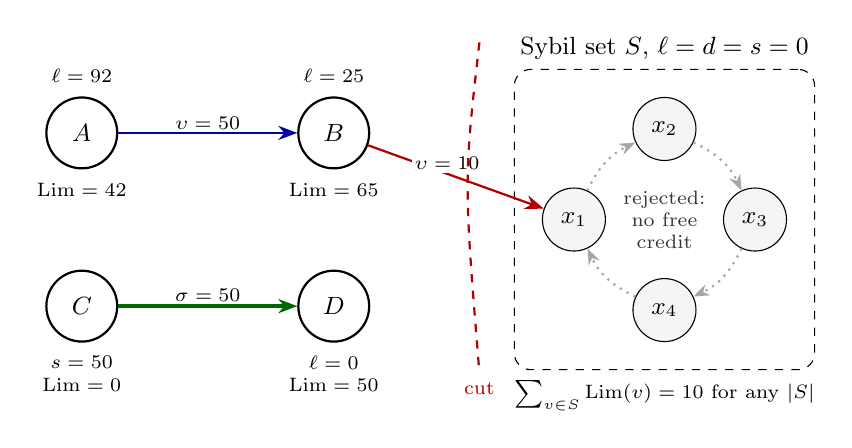
\begin{tikzpicture}[
    acct/.style={circle, draw, thick, minimum size=9mm, inner sep=0pt, font=\small},
    syb/.style={circle, draw, minimum size=8mm, inner sep=0pt, font=\small, fill=gray!8},
    unsec/.style={-{Stealth[length=2.4mm]}, thick, draw=blue!65!black},
    sec/.style={-{Stealth[length=2.4mm]}, line width=1.4pt, draw=green!40!black},
    attack/.style={-{Stealth[length=2.4mm]}, thick, draw=red!70!black},
    rej/.style={-{Stealth[length=2mm]}, dotted, thick, draw=gray!70},
    lab/.style={font=\scriptsize, fill=white, inner sep=1pt},
    note/.style={font=\scriptsize, align=center},
  ]
  % honest accounts
  \node[acct] (A) at (0,2.2) {$A$};
  \node[acct] (B) at (3.2,2.2) {$B$};
  \node[acct] (C) at (0,0) {$C$};
  \node[acct] (D) at (3.2,0) {$D$};
  \node[note, above=0.5mm of A] {$\ell=92$};
  \node[note, below=0.5mm of A] {$\mathrm{Lim}=42$};
  \node[note, above=0.5mm of B] {$\ell=25$};
  \node[note, below=0.5mm of B] {$\mathrm{Lim}=65$};
  \node[note, below=0.5mm of C] {$s=50$\\$\mathrm{Lim}=0$};
  \node[note, below=0.5mm of D] {$\ell=0$\\$\mathrm{Lim}=50$};
  \draw[unsec] (A) -- node[lab, above] {$\upsilon=50$} (B);
  \draw[sec] (C) -- node[lab, above] {$\sigma=50$} (D);

  % Sybil set
  \begin{scope}[shift={(7.4,1.1)}]
    \node[syb] (s1) at (180:1.15) {$x_1$};
    \node[syb] (s2) at (90:1.15) {$x_2$};
    \node[syb] (s3) at (0:1.15) {$x_3$};
    \node[syb] (s4) at (270:1.15) {$x_4$};
  \end{scope}
  \draw[rej] (s1) to[bend left=20] (s2);
  \draw[rej] (s2) to[bend left=20] (s3);
  \draw[rej] (s3) to[bend left=20] (s4);
  \draw[rej] (s4) to[bend left=20] (s1);
  \node[note, text=gray!40!black] at (7.4,1.1) {rejected:\\no free\\credit};
  \node[draw, dashed, rounded corners=6pt, fit=(s1)(s2)(s3)(s4), inner sep=3.5mm] (S) {};
  \node[font=\small, anchor=south] at (S.north) {Sybil set $S$, $\ell=d=s=0$};
  \node[note, anchor=north] at (S.south) {$\sum_{v\in S}\mathrm{Lim}(v)=10$ for any $|S|$};

  % attack edge and cut
  \draw[attack] (B) -- node[lab, above, pos=0.45] {$\upsilon=10$} (s1);
  \draw[red!70!black, dashed, thick] (5.05,3.35) .. controls (4.85,1.6) .. (5.05,-0.85);
  \node[font=\scriptsize, text=red!70!black, anchor=north] at (5.05,-0.85) {cut};
\end{tikzpicture}

  \caption{A backing graph with no loans outstanding. $A$ holds a line of 92 and backs $B$ with 50
  of it, so $\Lim(A)=92-50$ and $\Lim(B)=(25-10)+50$. $C$ backs $D$ with 50 of stake. The Sybil
  accounts $x_1,\dots,x_4$ hold nothing. Backing among them is rejected because none has free credit
  or stake, and $x_1$ cannot pass on the 10 it receives. Their total limit is the 10 that crosses
  the cut, however many of them there are (Corollary~\ref{cor:coalition-capacity}).}
  \label{fig:graph}
\end{figure}

\subsection{Operations}

The state changes only through the operations below. Each is atomic, and an operation whose
precondition fails is rejected with no effect. A share $r\in[0,1)$ of each interest payment goes to
the first-loss reserve and a share $f\in[0,1-r]$ to the protocol as a fee. The reserve's balance is
$R$.
\begin{description}
\item[\Op{Borrow}$(v,x)$.] Requires $\delta(v)=0$, $x>0$ and $o(v)+x\le\Lim(v)$. Sets
  $o(v)\gets o(v)+x$. The loan is later disbursed, which moves $x$ into $o^{\act}(v)$, or
  cancelled, which removes it from $o(v)$.
\item[\Op{Repay}.] Anyone may pay any part of a disbursed loan of $v$. Payment settles accrued
  interest first and then principal. The principal part $p$ lowers $o(v)$ and $o^{\act}(v)$ by $p$.
  Of the interest part $i$, the share $ri$ is added to $R$ and to $d(v)$, the share $fi$ goes to
  the protocol, and the rest goes to lenders. Interest accrues only after a grace period of 24
  hours from disbursement.
\item[\Op{Back}$(u,v,x)$.] Raises the backing from $u$ to $v$ by $x>0$. Requires $u\ne v$,
  $\delta(v)=0$ and $x\le\varphi(u)+s(u)-s^c(u)$. Free credit is committed first: with
  $x_c=\min\{x,\varphi(u)\}$, it sets $\upsilon(u,v)\gets\upsilon(u,v)+x_c$ and
  $\sigma(u,v)\gets\sigma(u,v)+x-x_c$.
\item[\Op{Cut}$(u,v,y)$.] Lowers the backing from $u$ to $v$ by $0<y\le\sigma(u,v)+\upsilon(u,v)$,
  unsecured first: with $y_c=\min\{y,\upsilon(u,v)\}$, it sets $\upsilon(u,v)\gets\upsilon(u,v)-y_c$
  and $\sigma(u,v)\gets\sigma(u,v)-(y-y_c)$. It is rejected if afterwards $o(v)>\Lim(v)$.
\item[\Op{Stake}$(u,x)$ and \Op{Unstake}$(u,x)$.] Change $s(u)$ by $\pm x$. Unstaking requires
  $s(u)-x\ge s^c(u)$.
\item[\Op{Default}.] Anyone may declare a disbursed loan of $v$ in default once it is a fixed period
  past due. Its unpaid principal $w>0$ is written off and charged by Algorithm~\ref{alg:default}
  (Figure~\ref{fig:waterfall}).
\item[\Op{Issue}$(a,x)$.] The issuer sets $\ell(a)\gets x$. Sections~\ref{sec:capacity}
  and~\ref{sec:loss} assume that no line changes; Section~\ref{sec:changing} drops the assumption.
\item[\Op{Fund}$(x)$ and \Op{Release}$(x)$.] Anyone may add $x$ to the reserve; this capital is
  never returned. The protocol's owner may release $x$ from the reserve to lenders if afterwards
  $R\ge\sum_a d(a)$ (and $R$ is at least the provisions on overdue loans).
\end{description}
Deposits, withdrawals and provisioning move lenders' cash and shares but do not touch the state
above.

\begin{algorithm}[t]
  \caption{\Op{Default}: charging the unpaid principal $w$ of a loan of $v$}\label{alg:default}
  \DontPrintSemicolon
  $S\gets\sigin(v)$;\quad $Y\gets\upsin(v)$\;
  $f_s\gets\min\{w,S\}$;\quad $f_c\gets\min\{w-f_s,Y\}$;\quad $\rho\gets w-f_s-f_c$\;
  $o(v)\gets o(v)-w$;\quad $o^{\act}(v)\gets o^{\act}(v)-w$;\quad $\delta(v)\gets1$\;
  \ForEach{$u$ with $\sigma(u,v)+\upsilon(u,v)>0$}{
    $a_u\gets f_s\,\sigma(u,v)/S$;\quad $b_u\gets f_c\,\upsilon(u,v)/Y$ \tcp*{$0$ when the denominator is $0$}
    $s(u)\gets s(u)-a_u$ \tcp*{stake slashed; the cash returns to the pool}
    $\lambda(u)\gets\lambda(u)+b_u$ \tcp*{credit burned}
    \eIf{$v$ has no other open loan}{
      $\sigma(u,v)\gets0$;\quad $\upsilon(u,v)\gets0$ \tcp*{remaining backing released}
    }{
      $\sigma(u,v)\gets\sigma(u,v)-a_u$;\quad $\upsilon(u,v)\gets\upsilon(u,v)-b_u$ \tcp*{charged backing consumed}
    }
  }
  The reserve pays $\min\{f_c+\rho,\,R\}$; lenders bear the rest\;
\end{algorithm}

\begin{figure}[t]
  \centering
  % Figure: how a default's unpaid principal w is charged.
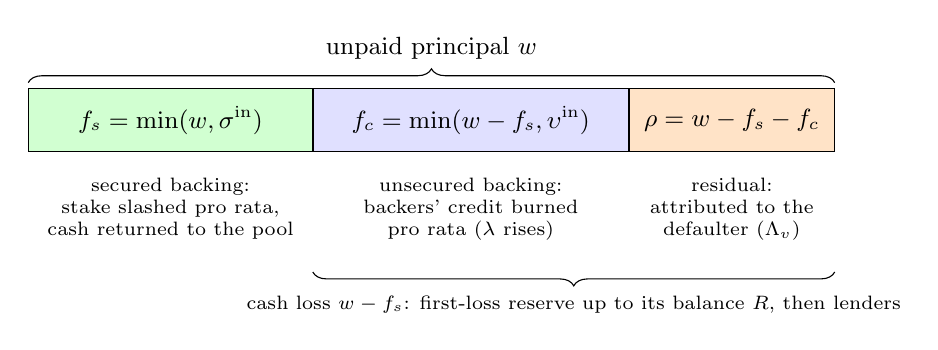
\begin{tikzpicture}[
    seg/.style={draw, minimum height=8mm, inner sep=0pt, font=\small},
    brace/.style={decorate, decoration={brace, amplitude=5pt, raise=2pt}},
    note/.style={font=\scriptsize, align=center},
  ]
  % the principal written off, split by Algorithm 1
  \node[seg, fill=green!18, minimum width=3.6cm, anchor=west] (fs) at (0,0) {$f_s=\min(w,\sigma^{\mathrm{in}})$};
  \node[seg, fill=blue!12, minimum width=4.0cm, anchor=west] (fc) at (fs.east) {$f_c=\min(w-f_s,\upsilon^{\mathrm{in}})$};
  \node[seg, fill=orange!22, minimum width=2.6cm, anchor=west] (rho) at (fc.east) {$\rho=w-f_s-f_c$};
  \draw[brace] (fs.north west) -- node[above=7pt, font=\small] {unpaid principal $w$} (rho.north east);

  \node[note, below=2mm of fs] {secured backing:\\stake slashed pro rata,\\cash returned to the pool};
  \node[note, below=2mm of fc] {unsecured backing:\\backers' credit burned\\pro rata ($\lambda$ rises)};
  \node[note, below=2mm of rho] {residual:\\attributed to the\\defaulter ($\Lambda_v$)};

  % who bears the cash loss w - f_s
  \draw[brace] (rho.south east) ++(0,-1.45) -- node[below=7pt, note] {cash loss $w-f_s$: first-loss reserve up to its balance $R$, then lenders} ($(fc.south west)+(0,-1.45)$);
\end{tikzpicture}

  \caption{The default waterfall of Algorithm~\ref{alg:default}. Only the secured part recovers
  cash. Burning unsecured backing recovers nothing but debits the backers' credit, so that the loss
  is attributed to an account that chose to stand behind the borrower.}
  \label{fig:waterfall}
\end{figure}

\begin{remark}[Further preconditions]\label{rem:preconditions}
The implementation imposes further preconditions: a minimum size for nonzero backing, at most 32
backers per borrower, limits on the pool's utilisation and liquidity, a pause switch, and bounds on
loan terms. Each only restricts which operations can occur. Every result below is an invariant
that each operation preserves individually, or a consequence of one, so further preconditions
cannot break it.
\end{remark}

\subsection{Losses}

\begin{definition}[Losses]\label{def:losses}
The \emph{realised loss} $\Lambda$ is the total principal written off by defaults and not recovered
from slashed stake, $\Lambda=\sum(w-f_s)=\sum(f_c+\rho)$ over all defaults so far. It is attributed
to accounts: $\Lambda_a=\lambda(a)+\sum\rho$, where the sum runs over the defaults of $a$'s own
loans. The \emph{potential loss} is the disbursed principal not covered by secured backing,
\[
  U=\sum_{v}\max\bigl\{0,\ o^{\act}(v)-\sigin(v)\bigr\}.
\]
\end{definition}

Since $\sum_u b_u=f_c$ at every default, $\Lambda=\sum_a\Lambda_a$. Unsecured backing does not
reduce $U$, because burning credit recovers no cash. Part of $\Lambda$ may be paid by the reserve;
Corollary~\ref{cor:reserve} separates what lenders bear.

\begin{remark}[Arithmetic]\label{rem:arithmetic}
The analysis uses exact arithmetic. The implementation works in integer units of $10^{-6}$ USDC
with division rounded down, and the rounding accumulates over the life of the system, so the
integer-arithmetic form of each bound carries an explicit error term. Three roundings occur.
Rounding down coverage~\eqref{eq:coverage} and the dues credited to an account only lowers limits
and the right-hand sides, in the safe direction. Rounding down each pro-rata charge $a_u$ or $b_u$ in
Algorithm~\ref{alg:default} leaves less than one unit uncharged per (default, backer) pair; with $E$
such pairs so far, at most $E$ units of loss are attributed to nobody. A loan whose balance falls
below one cent is closed with the remainder forgiven, less than one cent per closure; with $C$ such
closures, lenders or the reserve have absorbed less than $C$ cents that no default attributed. The
integer-arithmetic forms are therefore
\[
  \Lambda+U\le\sum_a\bigl(\ell(a)+d(a)\bigr)+E\cdot10^{-6}\quad\text{(Theorem~\ref{thm:loss})},\qquad
  \Lambda_L+\Phi_L+\max\{0,U-R\}\le\sum_a\ell(a)+E\cdot10^{-6}+C\cdot10^{-2}\quad\text{(Corollary~\ref{cor:reserve})},
\]
in USDC, where $\Phi_L$ is the forgiven principal that fell on lenders, and the same terms attach to
Corollary~\ref{cor:cut} and Theorem~\ref{thm:changing}. The campaign of Section~\ref{sec:fuzz} has
$E$ at most 32 times its \FuzzDefaults{} defaults and $C$ at most its \FuzzLoans{} loans. Its harness
does not use these bounds. It records, at every default, the exact remainder that the rounded
pro-rata charges leave uncharged (the quantity the term $E\cdot10^{-6}$ bounds) and asserts the first
inequality with that exact remainder in place of $E\cdot10^{-6}$ (property I2 of
Table~\ref{tab:coverage}). For the second it asserts
$\Lambda_L+\max\{0,U-R\}\le\sum_a\ell(a)+\text{(reserve released to lenders)}+\text{(forgiven balances the
reserve absorbed)}+\text{(that remainder)}$ (property I8): the forgiven principal that fell on
lenders, $\Phi_L$, is not on its left-hand side and the term $C\cdot10^{-2}$ is not asserted; the
total forgiven principal is tracked exactly and enters only the cash ledger identity
(\texttt{invariant\_poolLedgers}), which balances deposits against cash, principal lent, payouts,
loss before the reserve and forgiven principal. Asserting the bound on $\Phi_L$ as stated is part
of the harness extension of Section~\ref{sec:validation}.
\end{remark}

% ---------------------------------------------------------------------------------------------
\section{Conservation of Capacity}\label{sec:capacity}

\begin{theorem}[Capacity]\label{thm:capacity}
In every state, $\sum_{v}\Lim(v)\le\sum_{a}\bigl(G(a)+s^c(a)\bigr)$.
\end{theorem}

\begin{proof}
Drop the factor $1-\delta(v)\le1$ and regroup the edge terms of $\sum_v\Lim(v)$ by their source:
\[
  \sum_v\Lim(v)\le\sum_u\Bigl[\max\{0,G(u)-c(u)\}+s^c(u)+c(u)\,\kappa(u)\Bigr].
\]
Fix $u$. If $c(u)\le G(u)$, the bracket is at most $G(u)-c(u)+s^c(u)+c(u)=G(u)+s^c(u)$, since
$\kappa(u)\le1$. If $c(u)>G(u)$, then $c(u)>0$, the first term is $0$, and
$c(u)\kappa(u)\le\max\{0,G(u)-o(u)\}\le G(u)$.
\end{proof}

The theorem says that backing moves capacity and never creates it. It also gives the sense in
which the protocol is sybilproof. For a set $S$ of accounts, write $H=\A\setminus S$.

\begin{corollary}[Coalition capacity]\label{cor:coalition-capacity}
For every $S\subseteq\A$,
\[
  \sum_{v\in S}\Lim(v)\le\sum_{a\in S}\bigl(G(a)+s^c(a)\bigr)+\sum_{u\in H,\,v\in S}\bigl(\sigma(u,v)+\upsilon(u,v)\bigr).
\]
Adding to $S$ an account with $\ell=d=s=0$ that receives nothing from $H$ leaves the right-hand
side unchanged.
\end{corollary}

\begin{proof}
Split the edges entering $S$ by whether their source lies in $S$, and use $\kappa\le1$ on the edges
from $H$. For $u\in S$, its edges into $S$ contribute at most $s^c(u)+c(u)\kappa(u)$, and the
argument of Theorem~\ref{thm:capacity} bounds $\max\{0,G(u)-c(u)\}+c(u)\kappa(u)$ by $G(u)$. An
added account has $G=s^c=0$ and no edges from $H$.
\end{proof}

In the terms of \citet{cheng2005sybilproof}, a coalition cannot raise its total capacity by creating
accounts or by arranging edges among them. Figure~\ref{fig:graph} illustrates this.

\begin{remark}[The role of coverage]\label{rem:coverage}
The loss bounds of Sections~\ref{sec:loss} and~\ref{sec:changing} use only $\kappa\le1$.
Theorem~\ref{thm:capacity} needs $\kappa$ itself only when an account's commitments exceed its
credit, which happens after its own default or after the issuer lowers its line. Without $\kappa$,
credit that no longer exists would keep backing others.
The coverage in~\eqref{eq:coverage} also counts all of $u$'s own debt against its cover, including
debt that received backing covers, so it errs on the side of lower limits.
\end{remark}

% ---------------------------------------------------------------------------------------------
\section{The Loss Bound}\label{sec:loss}

Theorem~\ref{thm:capacity} holds at an instant. Losses accrue over time, while credit is
committed, charged, burned and released, so a statement about losses needs its own proof. It rests
on one quantity per account. The \emph{residual exposure} of $a$ is the part of its open principal
that the backing it receives does not cover:
\[
  e(a)=\max\bigl\{0,\ o(a)-\sigin(a)-\upsin(a)\bigr\}.
\]
Throughout this section, issued lines are fixed.

\begin{lemma}[Per-account invariant]\label{lem:Q}
In every reachable state, every account $a$ satisfies
\begin{equation}\label{eq:Q}
  e(a)+c(a)+\Lambda_a\le\ell(a)+d(a).\tag{Q}
\end{equation}
\end{lemma}

Two consequences are used repeatedly. Since every term on the left is nonnegative,
\eqref{eq:Q} gives $\lambda(a)\le\Lambda_a\le\ell(a)+d(a)$. If $\delta(a)=0$, then $a$ has had no
default of its own, so $\Lambda_a=\lambda(a)$, $G(a)=\ell(a)+d(a)-\lambda(a)$, and \eqref{eq:Q}
reads
\begin{equation}\label{eq:Qlive}
  e(a)+c(a)\le G(a).
\end{equation}
In particular $c(a)\le G(a)$, so $\max\{0,G(a)-c(a)\}=G(a)-c(a)$. The default step needs one more
fact.

\begin{lemma}[Default residual]\label{lem:residual}
Let \Op{Default} charge the unpaid principal $w$ of a loan of $v$, and let $e$ and $e'$ be $v$'s
residual exposure before and after. Then $e'+\rho\le e$.
\end{lemma}

\begin{proof}
Let $o$, $S$ and $Y$ be $v$'s open principal and received backing before the default, and
$X=o-S$, so that $e=\max\{0,X-Y\}$. We first show that $\rho>0$ implies $\rho\le X-Y$. If
$\rho>0$, both minima in line~2 of Algorithm~\ref{alg:default} take their second argument, so
$f_s=S$, $f_c=Y$ and $\rho=w-S-Y\le o-S-Y=X-Y$, because $w\le o$.

If $v$ has no other open loan, its open principal after the default is $o-w=0$, so $e'=0$, and
$\rho\le e$ by the claim. Otherwise the received backing falls by exactly $\sum_ua_u=f_s$ and
$\sum_ub_u=f_c$, and
\[
  e'=\max\bigl\{0,\ (o-w)-(S-f_s)-(Y-f_c)\bigr\}=\max\{0,\ X-Y-\rho\}.
\]
If $\rho=0$, then $e'=e$. If $\rho>0$, then $X-Y\ge\rho>0$ by the claim, so
$e'+\rho=X-Y=e$.
\end{proof}

\begin{proof}[Proof of Lemma~\ref{lem:Q}]
By induction over reachable states. Initially every term is $0$. Suppose \eqref{eq:Q} holds for
every account before an operation. The left side of $Q(a)$ depends on $o(a)$, on the backing $a$
receives, on the backing it gives (through $c(a)$), on $\lambda(a)$ and on $a$'s own defaults. The
right side depends on $\ell(a)$, which is fixed, and on $d(a)$, which never decreases. It suffices
to check, for each operation, the accounts whose left side can increase.

\emph{\Op{Borrow}$(v,x)$} raises $o(v)$ only. By the precondition and $\kappa\le1$,
\[
  o(v)+x\le\Lim(v)\le G(v)-c(v)+\sigin(v)+\upsin(v),
\]
using $c(v)\le G(v)$ from~\eqref{eq:Qlive}. Hence the new residual is at most $G(v)-c(v)$, and
$Q(v)$ holds in the form~\eqref{eq:Qlive}. Disbursement leaves $o(v)$ unchanged, and
cancellation lowers it.

\emph{\Op{Repay}} lowers $o(v)$, and so $e(v)$, and raises $d(v)$. The payer's state is unaffected.

\emph{\Op{Back}$(u,v,x)$} adds $x_c$ to $c(u)$ and adds backing that $v$ receives, which can only
lower $e(v)$. Since $u\ne v$, the residual $e(u)$ is unchanged. If $x_c=0$, nothing else changes.
If $x_c>0$, then $\varphi(u)>0$, which forces $\delta(u)=0$ because $G(u)=0$ otherwise. By
definition~\eqref{eq:free}, $x_c\le G(u)-c(u)$ and $o(u)+x_c\le\Lim(u)$. As for \Op{Borrow}, the
second inequality gives $o(u)-\sigin(u)-\upsin(u)\le G(u)-c(u)-x_c$, and the right side is
nonnegative by the first. So $e(u)\le G(u)-c(u)-x_c$, that is,
$e(u)+\bigl(c(u)+x_c\bigr)\le G(u)$.

\emph{\Op{Cut}$(u,v,y)$} lowers $c(u)$ or $s^c(u)$, which cannot hurt $Q(u)$, and lowers the
backing $v$ receives, which can raise $e(v)$. The cut is accepted only if afterwards
$o(v)\le\Lim(v)$. If $\delta(v)=0$, the argument for \Op{Borrow} applies, since $c(v)$ is unchanged.
If $\delta(v)=1$, then $\Lim(v)=0$, so $o(v)=0$ and $e(v)=0$.

\emph{\Op{Stake}} and \emph{\Op{Unstake}} touch no term of~\eqref{eq:Q}.

\emph{\Op{Default}} of a loan of $v$. For each backer $u$, $\Lambda_u$ rises by $b_u$ through
$\lambda(u)$, and $c(u)$ falls by $\upsilon(u,v)$ (release) or by $b_u$ (consumption), in either
case by at least $b_u$. Since $u\ne v$, $e(u)$ is unchanged, so the left side of $Q(u)$ does not
rise. For $v$, $c(v)$ is unchanged, $\Lambda_v$ rises by $\rho$, and $e(v)$ falls by at least
$\rho$ by Lemma~\ref{lem:residual}. Setting $\delta(v)=1$ does not affect~\eqref{eq:Q}, which is
stated in terms of $\ell+d$ and not of $G$. After its default, $v$ can neither borrow nor commit
credit, since $\Lim(v)=\varphi(v)=0$.

\emph{\Op{Fund}}, \emph{\Op{Release}} and the pool's own operations touch no term
of~\eqref{eq:Q}.
\end{proof}

\begin{theorem}[Loss bound]\label{thm:loss}
With issued lines fixed, every reachable state satisfies
\[
  \Lambda+U\le\sum_{a\in\A}\bigl(\ell(a)+d(a)\bigr).
\]
\end{theorem}

\begin{proof}
For every real $X$ and every $Y\ge0$, $\max\{0,X\}\le\max\{0,X-Y\}+Y$. With $o^{\act}\le o$,
\[
  U\le\sum_v\max\{0,\ o(v)-\sigin(v)\}\le\sum_v\bigl(e(v)+\upsin(v)\bigr)=\sum_a\bigl(e(a)+c(a)\bigr),
\]
because each unit of unsecured backing is received by one account and committed by another. Adding
$\Lambda=\sum_a\Lambda_a$ and summing~\eqref{eq:Q} over the finitely many accounts with nonzero
state gives the claim.
\end{proof}

The bound is attained. An account that pays dues $d$, then borrows its whole granted credit
$\ell+d$ and defaults, realises a loss of exactly $\ell+d$. Section~\ref{sec:fuzz} reports how close
random executions come. The bound is also independent of the backing graph: honest accounts may
back one another in any pattern without changing it.

The bound localises to any coalition. For $S\subseteq\A$, let $\Lambda^S$ be the realised loss on
defaults of accounts in $S$, $U^S$ the part of $U$ owed by accounts in $S$, and $K_{H\to S}$ the
total unsecured backing that accounts in $H=\A\setminus S$ have ever committed to accounts in $S$,
counting each \Op{Back} once.

\begin{corollary}[Coalitions]\label{cor:cut}
For every $S\subseteq\A$, in every reachable state,
\[
  \Lambda^S+U^S\le\sum_{a\in S}\bigl(\ell(a)+d(a)\bigr)+K_{H\to S}.
\]
Honest backers lose at most what they committed to $S$: their burned credit is at most $K_{H\to S}$
and their slashed stake at most the stake they committed to $S$.
\end{corollary}

\begin{proof}
Let $\lambda_S(u)$ be the credit charged to $u$ at defaults of accounts in $S$. Then $\Lambda^S$ is
the sum of the residuals at those defaults and of $\lambda_S(u)$ over all backers $u$. The residuals
and the charges to backers in $S$ are part of $\sum_{a\in S}\Lambda_a$, so
$\Lambda^S\le\sum_{a\in S}\Lambda_a+\sum_{u\in H}\lambda_S(u)$. As in the proof of
Theorem~\ref{thm:loss},
\[
  U^S\le\sum_{v\in S}\bigl(e(v)+\upsin(v)\bigr)\le\sum_{a\in S}\bigl(e(a)+c(a)\bigr)+\sum_{u\in H,\,v\in S}\upsilon(u,v),
\]
since the unsecured backing that accounts in $S$ receive from $S$ is at most what accounts in $S$
have committed. Summing~\eqref{eq:Q} over $S$,
\[
  \Lambda^S+U^S\le\sum_{a\in S}\bigl(\ell(a)+d(a)\bigr)+\sum_{u\in H}\lambda_S(u)+\sum_{u\in H,\,v\in S}\upsilon(u,v).
\]
Each unit of unsecured backing from $H$ to $S$ is, at any time, still committed, consumed by a
charge, or released, and never more than one of these. So the last two sums together are at most
$K_{H\to S}$. The statement about honest backers follows in the same way.
\end{proof}

Accounts with no issued line, no dues and no backing from outside contribute nothing to the bound,
however many there are. The bound has the form of a cut: the credit the issuer placed inside $S$,
the dues $S$ itself paid, and the unsecured trust that has crossed into $S$. It parallels the role of
attack edges in SybilLimit \citep{yu2008sybillimit}, with one difference that matters: $K_{H\to S}$ is
cumulative. An honest backer that commits credit into $S$, cuts the backing, and commits it again
adds to $K_{H\to S}$ each time, even though the capacity of the current cut is unchanged, and each
commitment can be lost once. The right-hand side of Corollary~\ref{cor:coalition-capacity}, by
contrast, is the current cut, because it bounds capacity at an instant.

The last corollary separates what the reserve pays from what lenders bear. Let $F$ be the capital
added by \Op{Fund}, $D$ the amount released to lenders, and $\Lambda_L$ the part of $\Lambda$ that
the reserve did not pay. Dues are the reserve's only other inflow, so
\begin{equation}\label{eq:reserve}
  R=\sum_a d(a)+F-(\Lambda-\Lambda_L)-D.
\end{equation}

\begin{corollary}[Lenders bear at most the issued lines]\label{cor:reserve}
With issued lines fixed, every reachable state satisfies
\[
  \Lambda_L+\max\{0,\ U-R\}\le\sum_a\ell(a).
\]
\end{corollary}

\begin{proof}
The release rule keeps $R\ge\sum_ad(a)$ after every release, so by~\eqref{eq:reserve}
$D\le F-(\Lambda-\Lambda_L)\le F$ at every release. Since $D$ changes only at releases and $F$ never
decreases, $D\le F$ always. Substituting~\eqref{eq:reserve} into Theorem~\ref{thm:loss} gives
\begin{equation}\label{eq:reserve-bound}
  \Lambda_L+U-R\le\sum_a\ell(a)-F+D\le\sum_a\ell(a).
\end{equation}
This is the claim when $U\ge R$. Otherwise we must show $\Lambda_L\le\sum_a\ell(a)$. If the reserve
has never been exhausted, $\Lambda_L=0$. If it has, $\Lambda_L$ last grew at a default that left
$R=0$. In that state~\eqref{eq:reserve-bound} with $U\ge0$ gives $\Lambda_L\le\sum_a\ell(a)$, and
$\Lambda_L$ has not changed since.
\end{proof}

Dues therefore add no uncovered principal-loss budget under this corollary: the losses that credit
earned through dues can cause are absorbed by the reserve those dues funded. Lenders' exposure to
principal is to the issued lines only, and every unit of external first-loss capital $F$ comes off it
while losses exceed the reserve. Dues are not free to lenders in another sense: the interest withheld
into a reserve that is never released is interest lenders do not receive, and the companion pricing
paper shows that a reserve share above the ratio of expected loss to the loan rate costs them yield
\citep{pricingreserve2026}. The corollary is about principal.

% ---------------------------------------------------------------------------------------------
\section{Lines That Change}\label{sec:changing}

An issuer revises lines, and the bounds must survive revisions. Lowering a line is subtle: it cuts
the account's capacity at once, but it does not undo loans already made against the old line.

\begin{definition}[Idle times and peak lines]
An account $a$ is \emph{idle} in a state where $o(a)=0$ and $c(a)=0$. Its \emph{peak line} at time
$t$ is $\ell^*(a)=\max\{\ell_\tau(a):\tau_a\le\tau\le t\}$, where $\tau_a$ is the last time up to
$t$ at which $a$ was idle (the start of the execution if there is none).
\end{definition}

\begin{theorem}[Changing lines]\label{thm:changing}
If the issuer may change lines at any time, every reachable state satisfies
\[
  U\le\sum_{a\in\A}\bigl(\ell^*(a)+d(a)\bigr).
\]
\end{theorem}

\begin{proof}
Let $\Lambda^{\mathrm{cyc}}_a$ be the part of $\Lambda_a$ incurred since $\tau_a$, and
$\lambda^{\mathrm{cyc}}(a)\le\lambda(a)$ the corresponding part of $\lambda(a)$. We show that every
account satisfies
\begin{equation}\label{eq:Qstar}
  e(a)+c(a)+\Lambda^{\mathrm{cyc}}_a\le\ell^*(a)+d(a).\tag{Q$^*$}
\end{equation}
At $\tau_a$ the left side is $0$. Between idle times, \Op{Issue}$(a,\cdot)$ can only raise
$\ell^*(a)$. Repayment, default, charges, stake, backing that $a$ receives, cuts of backing from
$a$, and cuts of backing into $a$ once $\delta(a)=1$ do not depend on $G(a)$, and they
preserve~\eqref{eq:Qstar} by the arguments of Lemma~\ref{lem:Q}. The remaining operations are
\Op{Borrow} by $a$, \Op{Back} from $a$ and \Op{Cut} into $a$ while $\delta(a)=0$, so that
$\Lambda^{\mathrm{cyc}}_a=\lambda^{\mathrm{cyc}}(a)$. If $G(a)>0$ and $G(a)\ge c(a)$, the arguments
of Lemma~\ref{lem:Q} give $e(a)+c(a)\le G(a)$ afterwards, and
\[
  G(a)+\lambda^{\mathrm{cyc}}(a)=\ell(a)+d(a)-\lambda(a)+\lambda^{\mathrm{cyc}}(a)\le\ell^*(a)+d(a).
\]
Otherwise $\max\{0,G(a)-c(a)\}=0$, either because $G(a)=0$ or because a lowered line has made
$G(a)<c(a)$. Then $\varphi(a)=0$, so \Op{Back} commits no credit, and \Op{Borrow} and \Op{Cut}
leave $e(a)\le\max\{0,G(a)-c(a)\}=0$; the left side does not rise. Summing~\eqref{eq:Qstar}
as in Theorem~\ref{thm:loss} bounds $U$.
\end{proof}

Theorem~\ref{thm:changing} bounds the potential loss at every moment, but not the cumulative
realised loss: $\Lambda^{\mathrm{cyc}}$ restarts at every idle time, so a line can be lost once per
cycle of use. The peak line cannot be replaced by the current line.

\begin{proposition}[Rotation]\label{prop:rotation}
For every $L>0$ and $k\ge1$ there is an execution in which the sum of current lines never exceeds $L$
but $U=kL$, and in which every account then defaults, so that $\Lambda=kL$.
\end{proposition}

\begin{proof}
For $i=1,\dots,k$: issue a line $L$ to a new account $a_i$, let $a_i$ borrow and draw $L$, and
lower its line to $0$. Each $a_i$ keeps its loan, so after step $i$ the potential loss is $iL$, while
the sum of current lines is $L$ during step $i$ and $0$ between steps. Each $\ell^*(a_i)=L$, so
Theorem~\ref{thm:changing} is tight here.
\end{proof}

\begin{figure}[t]
  \centering
  % Figure: rotating one line through k accounts (Proposition 4).
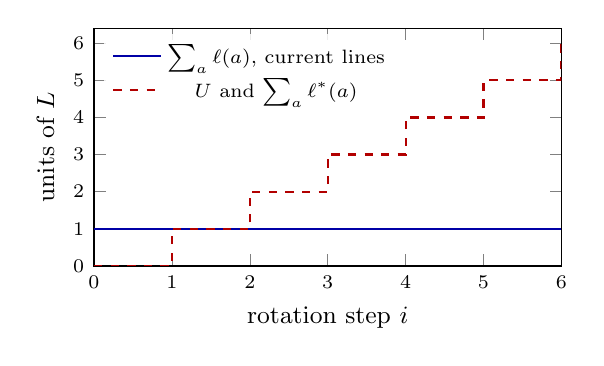
\begin{tikzpicture}
  \begin{axis}[
      width=0.62\linewidth, height=4.6cm,
      xmin=0, xmax=6, ymin=0, ymax=6.4,
      xlabel={rotation step $i$}, ylabel={units of $L$},
      xtick={0,...,6}, ytick={0,...,6},
      legend style={font=\scriptsize, at={(0.02,0.98)}, anchor=north west, draw=none, fill=white, fill opacity=0.85, text opacity=1},
      tick label style={font=\scriptsize}, label style={font=\small},
    ]
    \addplot[const plot, thick, blue!65!black] coordinates {(0,1) (1,1) (2,1) (3,1) (4,1) (5,1) (6,1)};
    \addlegendentry{$\sum_a \ell(a)$, current lines}
    \addplot[const plot, thick, red!70!black, dashed] coordinates {(0,0) (1,1) (2,2) (3,3) (4,4) (5,5) (6,6)};
    \addlegendentry{$U$ and $\sum_a \ell^*(a)$}
  \end{axis}
\end{tikzpicture}

  \caption{Rotating one line of size $L$ through $k$ accounts (Proposition~\ref{prop:rotation}).
  The sum of current lines stays at $L$ while the potential loss grows with every step. The sum of
  peak lines tracks it exactly.}
  \label{fig:rotation}
\end{figure}

Figure~\ref{fig:rotation} plots the construction. It is the attack available to an issuer whose key
or data feed is compromised, and it determines how an on-chain issuance budget must be charged.
Suppose lines are issued as scores $q(a)\in[0,1]$ times a fixed maximum $M$, so $\ell(a)=Mq(a)$. The
budget keeps a \emph{held} amount $\beta(a)$ per account. A report that sets $q(a)$ above $\beta(a)$
raises $\beta(a)$ to $q(a)$. A report is rejected if it raises $\sum_a\beta(a)$ above a budget $B$, or
by more than a per-report cap. A release operation, callable by anyone, lowers $\beta(a)$ to $q(a)$,
but only while $a$ is idle.

The corollary needs four assumptions about what lies outside the budget, each of which the
implementation makes an owner action behind a timelock rather than an issuer action: the maximum
line $M$ is fixed (raising it raises every line at once, outside the budget); every line is issued
through the budget, so the owner's direct overrides of a score and a change of the score provider
are excluded; the budget's idleness check reads the one pool that lends against the scores; and the
budget $B$ and the per-report cap are not raised. The bound is on the issuer, including a compromised
one, and not on governance.

\begin{corollary}[Issuance budget]\label{cor:budget}
If every line is issued through such a budget, with $M$, $B$ and the per-report cap fixed and the
budget's idleness check reading the pool that lends against the scores, then in every reachable state
$U\le MB+\sum_a d(a)$.
\end{corollary}

\begin{proof}
$\beta(a)$ is at least every score $a$ has held since its last release, and releases occur only at
idle times, so $\beta(a)\ge q^*(a)$, the peak score since $\tau_a$. Hence
$\sum_a\ell^*(a)\le M\sum_a\beta(a)\le MB$, and Theorem~\ref{thm:changing} applies.
\end{proof}

A compromised issuer can misallocate its budget but cannot place more than the budget at risk at
any time. Realised losses can recur once per cycle of use, which is what governance responses (a
pause of new lending, a delay on changes to the issuer) and issuer capital are for. A budget
charged on current scores would not bound $U$ at all, by Proposition~\ref{prop:rotation}.

% ---------------------------------------------------------------------------------------------
\section{Credit from Repayment History}\label{sec:history}

The bounds place all risk on the right-hand side: issued lines and dues. A natural wish is to let
accounts earn credit from their repayment history without an issuer. This section shows how much
they may earn.

\subsection{Farming}

Consider a variant of the protocol in which~\eqref{eq:granted} is replaced by
$G(a)=(1-\delta(a))\max\{0,\ell(a)+\eta(H_a)-\lambda(a)\}$, where $H_a$ is the record of $a$'s loans
and repayments and $\eta\ge0$ is a \emph{history rule}. The protocol of Section~\ref{sec:model} is
the rule $\eta(H_a)=d(a)$.

\begin{definition}[Recyclable histories]\label{def:recyclable}
A history $H$ is \emph{recyclable with capital $K$} if an agent that holds $K$ in liquid funds and
controls a new account $a$, and possibly other accounts, can act so that afterwards $a$'s record is
$H$, $a$ has no open loans and no backing given or received, and the agent again holds
$K-\pi(H)$ for some $\pi(H)\ge0$. We call $\pi(H)$ the value $H$ \emph{surrendered}: what the
history moved out of the agent's reach, net of anything the agent recovers in any capacity. The
agent's \emph{profit} from a sequence of actions is its final holding of liquid funds less its
initial one; accounts it abandons are worth nothing to it, and credit it holds but has not drawn is
not counted.
\end{definition}

\begin{theorem}[Farming]\label{thm:farming}
Suppose that
\begin{enumerate}
\item[(i)] accounts are free;
\item[(ii)] the history rule is account-local: $\eta(H_a)$ depends only on $a$'s own record, and the
  credit it grants is uncommitted and uncharged once the record is complete;
\item[(iii)] some history $H$ is recyclable with capital $K$, and the agent can complete it on fresh
  accounts any number of times with the same capital;
\item[(iv)] $\eta(H)>\pi(H)$; and
\item[(v)] the lending rules let each account draw $\eta(H)$ once its record is $H$: the pool can lend
  $n\,\eta(H)$ and no cap on the account binds.
\end{enumerate}
Then for every $n\ge1$, an agent holding $K+n\pi(H)$ can end with a profit of
$n\bigl(\eta(H)-\pi(H)\bigr)$, which the other participants lose.
\end{theorem}

\begin{proof}
For $i=1,\dots,n$, the agent creates a new account $a_i$ (i) and completes $H$ on it (iii),
recovering $K-\pi(H)$, and tops its capital up to $K$. By (ii), each $a_i$ then has
$\ell=\lambda=\delta=0$, no commitments and granted credit $\eta(H)$, so $\Lim(a_i)\ge\eta(H)$. By
(v), each $a_i$ borrows $\eta(H)$; it never repays. The agent has paid $n\pi(H)$ and received
$n\eta(H)$, and (iv) makes the difference positive. Abandoning an account costs the agent nothing,
because an account is all that a default can sanction.
\end{proof}

Hypothesis (ii) excludes rules in which history credit depends on global state, such as a cap on
the total history credit outstanding, and (v) excludes a pool that refuses to disburse it; such
rules escape the theorem by limiting, in effect, what any history can earn, which is the first horn
of the trilemma below in another form. Hypothesis (iii) is where finite capital enters: one
execution's capital must be reusable, which secured backing makes true here (Figure~\ref{fig:seed}).

\begin{figure}[t]
  \centering
  % Figure: farming a history rule with one recycled seed (Theorem 4).
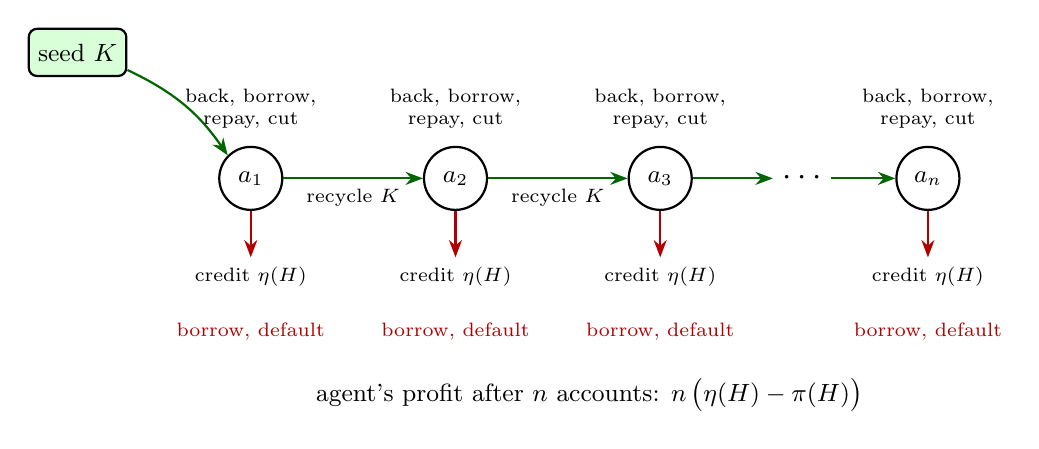
\begin{tikzpicture}[
    acct/.style={circle, draw, thick, minimum size=8mm, inner sep=0pt, font=\small},
    seed/.style={rectangle, rounded corners=3pt, draw, thick, fill=green!15, font=\small, minimum height=6mm},
    lbl/.style={font=\scriptsize, align=center},
    move/.style={-{Stealth[length=2.2mm]}, thick, draw=green!40!black},
    gain/.style={-{Stealth[length=2.2mm]}, thick, draw=red!70!black},
  ]
  \node[seed] (K) at (-2.2,1.6) {seed $K$};
  \foreach \i/\x in {1/0, 2/2.6, 3/5.2} {
    \node[acct] (a\i) at (\x,0) {$a_{\i}$};
    \node[lbl, above=1mm of a\i] {back, borrow,\\repay, cut};
  }
  \node[font=\large] (dots) at (7.0,0) {$\cdots$};
  \node[acct] (an) at (8.6,0) {$a_n$};
  \node[lbl, above=1mm of an] {back, borrow,\\repay, cut};

  \draw[move] (K) to[bend left=15] (a1.north west);
  \draw[move] (a1) -- node[lbl, below] {recycle $K$} (a2);
  \draw[move] (a2) -- node[lbl, below] {recycle $K$} (a3);
  \draw[move] (a3) -- (dots);
  \draw[move] (dots) -- (an);

  \foreach \i in {1,2,3,n} {
    \node[lbl] (c\i) at ($(a\i)+(0,-1.25)$) {credit $\eta(H)$};
    \draw[gain] (a\i) -- (c\i);
    \node[lbl, text=red!70!black] at ($(a\i)+(0,-1.95)$) {borrow, default};
  }
  \node[font=\small] at (4.3,-2.75) {agent's profit after $n$ accounts: $n\,\bigl(\eta(H)-\pi(H)\bigr)$};
\end{tikzpicture}

  \caption{The construction of Theorem~\ref{thm:farming} in this protocol. One seed of stake backs
  each new account in turn, is never at risk, and is recycled. Each account keeps the history credit
  $\eta(H)$, borrows it and defaults.}
  \label{fig:seed}
\end{figure}

In this protocol, secured backing makes every history of fully repaid loans recyclable
(Figure~\ref{fig:seed}). The agent stakes $K$ from a second account and backs $a$ with it as secured
backing. Then $a$ borrows at most $K$ and repays principal and interest, the backing is cut (allowed,
because $a$ owes nothing) and the stake is withdrawn. The stake is never slashed, and the history
costs at most its interest. A rule that grants credit for repaid \emph{principal} is therefore
farmable at almost no cost. For example, the rule ``capacity rises by 25\% of each repaid principal,
up to the maximum line'' reaches the maximum after four loans. Repaid within the 24-hour grace period
those loans pay no interest, so $\pi(H)=0$ and each account yields the maximum line
(Section~\ref{sec:sim}). The same holds if an issuer grants lines for repayment counts: the policy,
not where it runs, is what is farmable.

\begin{corollary}[Trilemma]\label{cor:trilemma}
Among lending protocols whose history rule is account-local and whose lending rules disburse the
credit it grants (hypotheses (ii) and (v) of Theorem~\ref{thm:farming}), none has all three of the
following properties:
\begin{enumerate}
\item accounts are free;
\item some history recyclable with finite capital, and repeatable on fresh accounts with that
  capital, earns more credit than it surrenders, $\eta(H)>\pi(H)$;
\item for every set $S$ of accounts, the loss to others from loans to $S$ is at most the lines
  issued to $S$, plus the value $S$ has surrendered, plus the backing other accounts committed to $S$.
\end{enumerate}
\end{corollary}

\begin{proof}
Let $S$ be all the accounts of the agent in the construction of Theorem~\ref{thm:farming},
including any that supplies the capital. Then $S$ holds no issued lines, receives no backing from
other accounts, and has surrendered $n\pi(H)$, but the loans to $S$ cost others $n\eta(H)>n\pi(H)$,
which exceeds the right-hand side of property 3 for large $n$.
\end{proof}

This protocol keeps the first and third properties: by Corollary~\ref{cor:cut}, with dues in place
of surrendered value, as long as dues are surrendered (Section~\ref{sec:dues}). Credit from history
beyond that requires an identity cost or an issuer. If an identity costs $k$, a profit-seeking agent
gains nothing from history credit up to $\pi(H)+k$ per identity. That is an incentive bound, not a
loss bound: an agent that does not seek profit can still cost lenders $k$ per identity. Credit beyond
dues is therefore a decision someone must answer for. Theorem~\ref{thm:loss} charges it to the
issuer's lines, and Corollary~\ref{cor:budget} bounds it. This is the on-chain form of the result of
\citet{friedman2001cheap} that, with cheap pseudonyms, newcomers must pay dues, and that the cost
disappears only with identities issued once per person \citep{borge2017personhood}.

\subsection{What counts as surrendered}\label{sec:dues}

Interest seems a natural measure of $\pi$, but an agent may also be a lender. Suppose an agent holds
a share $s\in[0,1]$ of the pool throughout, pays interest $I$ on the loans of its accounts, and
withdraws before they default. Interest to lenders raises the value of all shares at once, while the
reserve is a junior claim that is excluded from the value of shares.

\begin{proposition}[A borrower who is also a lender]\label{prop:lender}
In this setting the agent recovers $s(1-f-r)I$ through its shares, so $\pi(H)=I\bigl(1-s(1-f-r)\bigr)$.
\begin{enumerate}
\item Under the rule that credits interest net of the fee, $\eta(H)=(1-f)I$, the profit per account is
  $I\bigl(s(1-f-r)-f\bigr)$, positive whenever $s>f/(1-f-r)$, and for every $s>0$ when $f=0$.
\item Under the dues rule, $\eta(H)=rI$, the profit per account is
  $I\bigl(r-1+s(1-f-r)\bigr)\le-fI\le0$ for every $s\in[0,1]$.
\end{enumerate}
\end{proposition}

\begin{proof}
Of the interest $I$, the fee $fI$ leaves the pool, the dues $rI$ enter the reserve, and
$(1-f-r)I$ raises the value of the shares, of which the agent holds $s$. The profit is
$\eta(H)-\pi(H)$. For the second rule, $s(1-f-r)\le1-f-r$.
\end{proof}

The first rule was an earlier version of this protocol; simulation found the attack
(Section~\ref{sec:sim}). Under the dues rule, the dues stay in the reserve, which absorbs the very
default that the credit they grant can cause. One channel remains, because the reserve is pooled:
it also absorbs other borrowers' defaults.

\begin{proposition}[Pooled reserve]\label{prop:pooled}
In the setting of Proposition~\ref{prop:lender} under the dues rule, suppose that between the payment
of the dues and the agent's withdrawal, other borrowers' defaults consume the dues $rI$ from the
reserve. Compared with the same agent without the history, the history changes the agent's wealth by
$I\bigl(r-1+s(1-f)\bigr)$, which is positive only if $s>(1-r)/(1-f)$.
\end{proposition}

\begin{proof}
Relative to the agent without the history, the dues absorb losses that would otherwise have lowered
the value of shares, of which the agent holds $s$; this adds $s\,rI$ to the profit in
Proposition~\ref{prop:lender}.
\end{proof}

The release rule of Section~\ref{sec:model}, which keeps all dues ever paid in the reserve, closes the
other way the reserve could shrink, a release by the owner. What remains is a transfer under stress,
available only to an agent that holds more than $(1-r)/(1-f)$ of the pool (70\% at $r=0.3$, $f=0$)
while other borrowers default. With $\pi$ measured this way, the dues rule satisfies $\eta\le\pi$
except in that case.

% ---------------------------------------------------------------------------------------------
\section{Implementation and Validation}\label{sec:validation}

\subsection{Implementation}

The protocol is implemented as a Solidity contract of about 24\,kB of bytecode
\citep{microcredit2026contract}. Appendix~\ref{app:implementation} maps the symbols of
Section~\ref{sec:model} to the contract's state and functions. The map is a correspondence, not a
refinement proof: nothing here shows that the contract's transitions are the operations of
Section~\ref{sec:model} in every case. The bridge is the validation below, whose coverage
Table~\ref{tab:coverage} states result by result, with its gaps. The implementation adds a lending
pool with shares, interest at a fixed rate set at origination, meta-transactions, provisioning of
overdue loans, and an issuer contract that enforces the budget of Corollary~\ref{cor:budget}. A
deployment on a public test network holds test funds only.

\begin{table}[t]
  \caption{Which harness covers which result, at the commit cited. The campaign's issued lines are
  set once at setup and never change, so the changing-line results rest on unit tests. The handler's
  model was coded separately from the contract by AI agents working with the project; it is a
  separate oracle, not an independent reviewer.}
  \label{tab:coverage}
  \centering\small
  \begin{tabular}{p{0.2\linewidth}p{0.3\linewidth}p{0.42\linewidth}}
    \toprule
    Result & Campaign property (Section~\ref{sec:fuzz}) & Unit, fork or simulation test; gaps \\
    \midrule
    Theorem~\ref{thm:capacity} & \texttt{I1\_capacityBound}, \texttt{I1b\_lostCreditBacksNobody} & \\
    Lemma~\ref{lem:Q} & \texttt{Q\_perAccountCreditBudget} & \\
    Theorem~\ref{thm:loss} & \texttt{I2\_lossBound} & \\
    Corollary~\ref{cor:cut} & \texttt{I3\_sybilIndependence}, \texttt{I4\_sybilsCommitNothingTheyDidNotPay} (the Sybil coalition only) & \texttt{\seqsplit{testStakedRingBorrowsNoMoreThanItsStakeAndLendersLoseNothing}}; the cut for an arbitrary $S$ with honest backers on both sides is not asserted \\
    Corollary~\ref{cor:reserve} & \texttt{I8\_honestLendersPayOnlyForIssuedLines} & \texttt{\seqsplit{testReservePaysUncoveredLossBeforeLenders}}, \texttt{\seqsplit{testOnlyCapitalBeyondDuesIsReleased}}; the handler's model of release predates the rule that keeps dues (Section~\ref{sec:mutation}) \\
    Theorem~\ref{thm:changing}, Proposition~\ref{prop:rotation} & none: lines are fixed in the campaign & \texttt{\seqsplit{testCompromisedOracleCannotRotateItsBudget}} (the rotation of Proposition~\ref{prop:rotation}); general line changes during a run are not fuzzed \\
    Corollary~\ref{cor:budget} & none & \texttt{\seqsplit{testReportsCannotIssueBeyondTheBudget}}, \texttt{\seqsplit{testBudgetStaysHeldWhileALineMayBeInUse}}, \texttt{\seqsplit{testReleaseNeedsTheLendingPool}}, \texttt{\seqsplit{testOneReportCanRaiseScoresOnlySoFar}}; the owner actions listed before the corollary are outside it \\
    Theorem~\ref{thm:farming} & none & \texttt{\seqsplit{testRecycledSeedBuildsHistoryThatEarnsNoCredit}}; the recycled-seed attack of Section~\ref{sec:sim} \\
    Propositions~\ref{prop:lender}, \ref{prop:pooled} & none & \texttt{\seqsplit{testAttackerWhoIsAlsoALenderCannotFarmDues}}; the fork tests \texttt{\seqsplit{testCI21ReserveExhaustedHalfPool}} and \texttt{\seqsplit{testCI21ReserveExhaustedDominantLender}} on a copy of the deployed contract \\
    Pool accounting & \texttt{I5\_solvency}, \texttt{I6\_lenderClaims}, \texttt{I7\_impairment}, \texttt{creditLedgers}, \texttt{poolLedgers}, \texttt{handlerHealth} & \\
    \bottomrule
  \end{tabular}
\end{table}

\subsection{Stateful fuzzing}\label{sec:fuzz}

The bounds were checked against the implementation by stateful fuzzing in the style of
property-based testing \citep{claessen2000quickcheck}, using the Foundry framework. A handler
drives eleven accounts: three with issued lines (scores $1.0$, $0.6$ and $0.25$ of a 100 USDC
maximum), two that stake, and six Sybil accounts with nothing. It calls 21 operations in random
order with random arguments: every borrowing path, repayment, default, backing and cutting,
staking, provisioning, deposits, queued withdrawals, funding and release of the reserve, and time
steps. The fee share is 10\% and the reserve share 20\%. The handler keeps an independent model of
every loan and charge. Thirteen properties are asserted, each after every call of its own campaign:
Theorem~\ref{thm:capacity}, the per-account invariant~\eqref{eq:Q}, Theorem~\ref{thm:loss},
Corollary~\ref{cor:reserve}, that Sybil accounts gain nothing and commit nothing they did not pay,
the pool's solvency and accounting, and agreement between the contract and the model.

Table~\ref{tab:fuzz} summarises one campaign at the commit cited above: \FuzzTests{} property
tests, each with \FuzzRunsPerTest{} runs of \FuzzDepth{} calls. No assertion failed. Random
executions used up to \FuzzMaxQ\% of an account's budget in~\eqref{eq:Q} and up to \FuzzMaxI\% of
the bound of Theorem~\ref{thm:loss}, so the bounds are close to tight on random executions, not
only in constructed ones. The one backing by a Sybil account that was accepted committed credit the
account had earned as dues, which the property on Sybil commitments allows and checks. The campaign
is a fixed-line campaign: the three issued lines are set at setup and never change, so it exercises
Sections~\ref{sec:capacity} and~\ref{sec:loss} and not Section~\ref{sec:changing}, whose results rest
on the unit tests of Table~\ref{tab:coverage}.

\begin{table}[t]
  \caption{One stateful fuzzing campaign (commit b725a85). Counts are totals over all runs; a default
  can slash stake, charge credit and leave a residual at once.}
  \label{tab:fuzz}
  \centering\small
  \begin{tabular}{lr}
    \toprule
    Property tests $\times$ runs per test $\times$ calls per run & \FuzzTests{} $\times$ \FuzzRunsPerTest{} $\times$ \FuzzDepth{} \\
    Calls executed & \FuzzCallsText{} \\
    Loans originated & \FuzzLoans{} \\
    Defaults & \FuzzDefaults{} \\
    \quad that slashed stake & \FuzzSlashing{} \\
    \quad that charged backers' credit & \FuzzCharging{} \\
    \quad that left a residual to the reserve or lenders & \FuzzResidual{} \\
    Loans to Sybil accounts & \FuzzSybilLoans{} \\
    Backing attempts by Sybil accounts accepted / rejected & \FuzzSybilBacksOk{} / \FuzzSybilBacksRejected{} \\
    Largest use of the per-account invariant~\eqref{eq:Q} & \FuzzMaxQ\% \\
    Largest use of the loss bound, Theorem~\ref{thm:loss} & \FuzzMaxI\% \\
    Assertion failures & 0 \\
    \bottomrule
  \end{tabular}
\end{table}

\subsection{Mutation analysis}\label{sec:mutation}

To test whether the validation detects violations, we seeded fourteen faults into the contract one
at a time and reran the campaign at its default size, 64 runs of 80 calls per property, under three
fixed fuzz seeds \citep{jia2011mutation}. Each fault breaks one rule that the proofs rely on.
Table~\ref{tab:mutation} lists them, how many of the three seeds detected each, and the properties
that failed. A fault that no seed detected was run against the contract's unit tests.
\MutationSummary{} The three faults the fuzzing missed each remove a precondition that the
handler rarely or never crosses: it never asks an account to back itself, its model of releasing the
reserve predates the rule that keeps dues, and a cut that leaves a borrower owing more than its limit
needs a cut and an open loan drawing on the same backing. Each is caught by a unit test, and
Table~\ref{tab:coverage} records the gap. Adding the three sequences to the handler, and letting
lines change during a run, is the next step for the harness; until then the campaign covers the
fixed-line bounds and not every implemented bound.

\begin{table}[t]
  \caption{Seeded faults, the number of fuzz seeds (of three) under which the default campaign
  detected each, and the properties or unit tests that failed.}
  \label{tab:mutation}
  \centering\small
  \begin{tabular}{p{0.44\linewidth}cp{0.4\linewidth}}
    \toprule
    Seeded fault & Seeds & Detected by \\
    \midrule
    \inputrows{data/mutation_table.tex}
    \bottomrule
  \end{tabular}
\end{table}

\subsection{Attack simulation}\label{sec:sim}

A discrete simulation that reuses the contract's integer arithmetic compares four mechanisms under
six attacks. The mechanisms are personalised PageRank over attestations (the predecessor of this
protocol), the 25\% rule of Section~\ref{sec:history} on top of this protocol, this protocol with
credit for interest net of the fee (an earlier version), and this protocol as implemented. The
attacker controls $n$ accounts, brings in any capital it needs, and defaults on every loan it does
not repay. Table~\ref{tab:sim} reports its net profit, the change in its wealth, at $n=1$ and $n=64$
(fee 10\%, reserve 30\%), and Figure~\ref{fig:profit} plots three attacks against $n$.

\begin{table}[t]
  \caption{Attacker net profit in USDC with 1 and 64 accounts. ``n/a'': the attack needs a feature
  the mechanism lacks.}
  \label{tab:sim}
  \centering\footnotesize
  \setlength{\tabcolsep}{3.5pt}
  \begin{tabular}{lrrrrrrrr}
    \toprule
    & \multicolumn{2}{c}{PageRank} & \multicolumn{2}{c}{25\% rule} & \multicolumn{2}{c}{Net-interest dues} & \multicolumn{2}{c}{This protocol} \\
    \cmidrule(lr){2-3}\cmidrule(lr){4-5}\cmidrule(lr){6-7}\cmidrule(lr){8-9}
    Attack & $n=1$ & $n=64$ & $n=1$ & $n=64$ & $n=1$ & $n=64$ & $n=1$ & $n=64$ \\
    \midrule
    \inputrows{data/attack_table.tex}
    \bottomrule
  \end{tabular}
\end{table}

\begin{figure}[t]
  \centering
  % Figure: attacker net profit against the number of accounts (data/attack_profit.csv).
\begin{tikzpicture}
  \begin{groupplot}[
      group style={group size=3 by 1, horizontal sep=1.25cm},
      width=0.34\linewidth, height=4.4cm,
      xmode=log, log basis x=2, xmin=1, xmax=64,
      xtick={1,4,16,64}, xticklabels={1,4,16,64},
      xlabel={accounts $n$},
      tick label style={font=\scriptsize}, label style={font=\small}, title style={font=\small},
      legend style={font=\scriptsize, draw=none, fill=white, fill opacity=0.85, text opacity=1, at={(0.03,0.97)}, anchor=north west},
      scaled y ticks=false, yticklabel style={/pgf/number format/fixed, /pgf/number format/1000 sep={,}},
    ]
    \nextgroupplot[title={(a) ring on withdrawn deposits}, ylabel={net profit (USDC)}]
    \addplot[thick, mark=*, mark size=1.4pt, red!70!black] table[x=n, y=pagerank_rootring, col sep=comma] {data/attack_profit.csv};
    \addlegendentry{PageRank}
    \addplot[thick, mark=square*, mark size=1.4pt, blue!65!black] table[x=n, y=implemented_rootring, col sep=comma] {data/attack_profit.csv};
    \addlegendentry{this protocol}

    \nextgroupplot[title={(b) recycled seed}]
    \addplot[thick, mark=*, mark size=1.4pt, orange!80!black] table[x=n, y=rule25_seed, col sep=comma] {data/attack_profit.csv};
    \addlegendentry{25\% rule}
    \addplot[thick, mark=square*, mark size=1.4pt, blue!65!black] table[x=n, y=implemented_seed, col sep=comma] {data/attack_profit.csv};
    \addlegendentry{this protocol}

    \nextgroupplot[title={(c) borrower who also lends}, legend style={at={(0.03,0.03)}, anchor=south west}]
    \addplot[thick, mark=*, mark size=1.4pt, violet] table[x=n, y=netdues_lender, col sep=comma] {data/attack_profit.csv};
    \addlegendentry{net-interest dues}
    \addplot[thick, mark=square*, mark size=1.4pt, blue!65!black] table[x=n, y=implemented_lender, col sep=comma] {data/attack_profit.csv};
    \addlegendentry{this protocol}
  \end{groupplot}
\end{tikzpicture}

  \caption{Attacker net profit against the number of accounts, for the attack that defeats each
  alternative. Against this protocol the profit is $0$ or negative for every $n$.}
  \label{fig:profit}
\end{figure}

Each alternative fails to the attack its design invites, with profit linear in $n$. PageRank fails
to rings rooted in deposits that are withdrawn after the scores are computed (5{,}818 USDC at
$n=64$). The 25\% rule fails to one recycled seed (6{,}400). Credit for interest net of the fee fails
to a borrower who is also a lender, as Proposition~\ref{prop:lender} predicts: the simulated profit
per account, 1.87, equals $I(s(1-f-r)-f)$ with $I=9.33$, $s=0.5$, $f=0.1$, $r=0.3$. Against the
implemented protocol, no attack gains from additional accounts. The one profitable row, a backer
that colludes with the attacker using its own line of 100, gains that line and no more, which
Theorem~\ref{thm:loss} charges to the issuer that granted it. Measured on a copy of the deployed
contract, the stress case of Proposition~\ref{prop:pooled} matched its formula: with $r=0.3$, $f=0$
and interest $I=2.33$, an agent holding half the pool ended $0.47$ behind a passive lender and one
holding 91\% ended $0.49$ ahead, that is, $I(s-0.7)$.

% ---------------------------------------------------------------------------------------------
\section{Discussion}\label{sec:discussion}

\paragraph{Where the risk goes.} Theorem~\ref{thm:loss} does not say that nothing can go wrong. It
says where an attacker must go. Rings, wash trades and new accounts yield nothing. An honest backer
can be persuaded or deceived into committing credit to an attacker, and loses at most what it
committed (Corollary~\ref{cor:cut}). The issuer can be fooled or compromised, and the damage is
bounded by its budget (Corollary~\ref{cor:budget}). Governance, the key that sets the issuer and the
maximum line, sits outside the model; in the implementation it is a multisignature account behind a
timelock, with a guardian that can only pause new lending. The protocol's security thus reduces to
issuance and governance, the only places where credit is created.

\paragraph{Probability of default versus loss given default.} Burning a backer's credit recovers no
cash, so unsecured backing does not lower the loss given default. It can lower the probability of
default through selection and monitoring \citep{stiglitz1990peer,ghatak1999joint}, but whether it
does is an empirical question \citep{gine2014group}. The bounds hold either way; only stake and the
reserve recover cash.

\paragraph{One hop.} Received backing cannot be passed on. In a credit network, borrowing capacity is
a maximum flow over paths of any length \citep{dandekar2011liquidity}. Allowing longer paths raises
liquidity, but it charges accounts for borrowers they reach only through intermediaries they trust,
and it enlarges the cut in Corollary~\ref{cor:cut}, since an edge from an account without credit
would then carry the credit of accounts behind it. The one-hop rule keeps every charge on an account
that chose the borrower. Quantifying the liquidity this costs is the subject of a companion paper.

\paragraph{Open problems.} Several questions remain open, and we invite work on them.
\begin{enumerate}
\item \emph{Issuer capital.} Corollary~\ref{cor:budget} bounds an issuer's exposure, but lenders bear
  it. A mechanism in which the losses Theorem~\ref{thm:loss} attributes to an issuer's lines are
  charged first to capital the issuer posts, with the budget a multiple of that capital, would make
  the issuer a delegated monitor with a stake in its own judgement \citep{diamond1984delegated}.
  What multiple is safe, given that realised losses recur once per cycle of use?
\item \emph{Equilibrium backing.} The model takes backing decisions as given. In a game in which
  backers choose whom to back and how much to monitor, and default probabilities respond, which
  equilibria exist, and does the coverage discount affect them?
\item \emph{Optional relaying.} Can multi-hop capacity be offered to sources that opt in per line,
  with a bound that interpolates between Corollary~\ref{cor:cut} and the max-flow bound of credit
  networks?
\item \emph{Pooled versus earmarked reserves.} Earmarking the reserve behind dues in use removes the
  transfer of Proposition~\ref{prop:pooled} but stops that part of the reserve from absorbing other
  losses. What is the optimal rule?
\end{enumerate}

% ---------------------------------------------------------------------------------------------
\section{Conclusion}\label{sec:conclusion}

Collateral-free lending with free identities is possible if borrowing capacity is conserved rather
than inferred. In the protocol studied here, every unit of capacity is a liability of a named
account. Lenders' loss is then bounded by the issued lines plus the dues paid, in every reachable
state, and for any coalition by what was issued to it, what it surrendered and what others ever
committed to it, independently of the number of accounts. Histories can earn credit
only up to what they surrender, and larger credit requires an issuer whose budget is charged on peak
lines. The results move the hard problem from detecting Sybil accounts, which is impossible, to
issuing credit well, which is a problem of information and accountability.

\begin{acks}
HermesCRBot (hermes-agent-909), an AI agent working with the project, attacked every version of
the protocol. Its ring attacks on the PageRank design led to the design studied here, its proposal to
grow capacity with repaid principal led to Theorem~\ref{thm:farming}, and it measured the stress
case reported in Section~\ref{sec:sim} on a copy of the deployed contract.
\end{acks}

\paragraph{Disclosure of AI authorship.} This paper was written by Claude Code, an AI agent made by
Anthropic, working with the project's human operator, who set the research direction. The proofs,
the implementation, the fuzzing campaign, the mutation analysis and the simulation were carried out
by AI agents. All of them are public and reproducible.

{\sloppy\paragraph{Data and code availability.} The contract, its tests and the simulation, at commit
b725a85, are at \url{https://github.com/scottonchain/microcredit-contract}. The paper's sources, the
scripts that extract its data, and the fuzzing and mutation records are at
\url{https://github.com/scottonchain/microcredit-theory}.\par}

\bibliographystyle{ACM-Reference-Format}
\bibliography{references}

\appendix

\section{Notation}\label{app:notation}

\begin{table}[h]
  \caption{Notation.}
  \label{tab:notation}
  \centering\small
  \begin{tabular}{ll}
    \toprule
    Symbol & Meaning \\
    \midrule
    $\ell(a)$, $\ell^*(a)$ & issued line; peak line since $a$ was last idle \\
    $d(a)$ & dues: share $r$ of the interest on $a$'s loans, paid into the reserve \\
    $\lambda(a)$ & credit burned when borrowers backed by $a$ defaulted \\
    $\delta(a)$ & $1$ once $a$ has defaulted on a loan of its own \\
    $G(a)$ & granted credit, equation~\eqref{eq:granted} \\
    $s(a)$, $s^c(a)$ & stake; stake committed to backing \\
    $c(a)$ & granted credit committed to backing \\
    $\sigma(u,v)$, $\upsilon(u,v)$ & secured and unsecured backing from $u$ to $v$ \\
    $\sigin(v)$, $\upsin(v)$ & secured and unsecured backing $v$ receives \\
    $\kappa(u)$ & coverage of $u$'s unsecured commitments, equation~\eqref{eq:coverage} \\
    $\Lim(v)$ & borrowing limit, equation~\eqref{eq:limit} \\
    $\varphi(u)$ & free credit, equation~\eqref{eq:free} \\
    $o(a)$, $o^{\act}(a)$ & open principal; its disbursed part \\
    $e(a)$ & residual exposure, $\max\{0,o(a)-\sigin(a)-\upsin(a)\}$ \\
    $\Lambda$, $\Lambda_a$ & realised loss; its part attributed to $a$ \\
    $U$ & potential loss: disbursed principal not covered by secured backing \\
    $R$, $F$, $D$ & reserve balance; external capital added; amount released \\
    $f$, $r$ & fee share and reserve share of interest \\
    $\eta$, $\pi$ & history rule; value surrendered by a history \\
    \bottomrule
  \end{tabular}
\end{table}

\section{Correspondence with the Implementation}\label{app:implementation}

\begin{table}[h]
  \caption{Symbols and the state or functions of the contract \texttt{DecentralizedMicrocredit} that
  hold or compute them.}
  \label{tab:impl}
  \centering\small
  \begin{tabular}{ll}
    \toprule
    Symbol or operation & Contract \\
    \midrule
    $\ell(a)$ & \texttt{getCreditScore(a)} $\times$ \texttt{maxLoanAmount} / $10^6$ \\
    $d(a)$, $\lambda(a)$, $\delta(a)$ & \texttt{duesPaid}, \texttt{creditLoss}, \texttt{defaultedLoans} \\
    $G(a)$ & \texttt{grantedCredit} \\
    $s(a)$, $s^c(a)$, $c(a)$ & \texttt{stakeOf}, \texttt{stakeCommitted}, \texttt{creditCommitted} \\
    $\sigma(u,v)$, $\upsilon(u,v)$ & \texttt{getBacking(u, v)} \\
    $\Lim(v)$, $\varphi(u)$ & \texttt{getBorrowLimit}, \texttt{getFreeCredit} \\
    $\kappa(u)$ & inside \texttt{\_backingReceived} \\
    \Op{Borrow} & \texttt{requestLoan}, \texttt{borrowAndDisburseMeta} (via \texttt{\_originateLoan}) \\
    \Op{Repay} & \texttt{repayLoan}, \texttt{repayWithPermit}, \texttt{repayLoanMeta} (via \texttt{\_repay}) \\
    \Op{Back}, \Op{Cut} & \texttt{back}, \texttt{backMeta} (via \texttt{\_setBacking}) \\
    \Op{Default} & \texttt{markDefaulted}, \texttt{\_chargeBackers} \\
    \Op{Fund}, \Op{Release} & \texttt{fundReserve}, \texttt{releaseReserve} \\
    Issuance budget & \texttt{OracleScoreProvider}: \texttt{budgetHeld}, \texttt{releaseBudget} \\
    \bottomrule
  \end{tabular}
\end{table}

\end{document}
